% =============================================================================
% ACT II — THE MEASUREMENT PROBLEM (Section 5)
% Restructured from results_format_dependence_v3.tex + results_final.tex
% Section 5.2 (option-preserving) moved here per Amendment A1
% Section 5.3 (reframing synthesis) is NEW content
% Section 5.4 (negative control reinterpreted) is NEW content
% =============================================================================

\section{The Measurement Problem}
\label{sec:measurement-problem}

The preceding section's results implicate the measurement instrument rather than underlying alignment.  AI factual recall remains immune despite running through the same format and scaffolds, while map-reduce degradation concentrates on MC-format benchmarks; option-preserving map-reduce recovers 40 to 89\% of the effect.  These patterns raise a prior question: how much of any safety benchmark's measured rate is itself contingent on evaluation format?

% ---------------------------------------------------------------------------
\subsection{Format Dependence of Safety Benchmarks}
\label{sec:format-dependence}

\paragraph{Overview.}
Experiment~5 tests format dependence directly: 220 matched item pairs administered in both MC and open-ended (OE) formats under both direct API and map-reduce, across five models ($N = 4{,}400$ observations, zero errors).  Crossing format with scaffold isolates how each contributes independently and how the two interact.

When format is held constant, scaffold effects vanish.  The within-format scaffold contrast is typically ${<}2$~pp on the 2$\times$2 design, TOST-equivalent within the pre-registered $\pm 2$~pp margin.  Most of the map-reduce degradation documented in Act~I is a format-conversion effect, not an alignment effect.  MMLU inflates measured capability by $9.2$~pp in MC versus OE; AI factual recall shows no format effect ($-1.0$~pp).

The format study uses 220 matched item pairs that are unevenly distributed across the five benchmarks (BBQ 60, TruthfulQA 60, sycophancy 20, AI factual recall 30, and MMLU 50, totalling 220 pairs); when paired with five models and two deployment configurations, this design yields cell sizes of 20 to 60 observations per model$\times$benchmark$\times$format combination (with $N = 4{,}400$ observations in total).  Power therefore varies accordingly across the different benchmarks.  For the smallest cells in the design, the minimum detectable effect at 80\% power is approximately 16~pp; for the largest cells, it is approximately 9~pp.  The observed effects on the affected safety benchmarks (which range from 5 to 20~pp) lie at or above these thresholds, with the corresponding achieved power for the BBQ ($+16.2$~pp) and sycophancy ($+19.6$~pp) effects both exceeding 0.99 at their respective cell sizes.  The AI factual recall null ($-1.0$~pp) falls below the minimum detectable effect and should therefore be interpreted as a failure to reject the null, not as proven equivalence; the same applies to the within-format scaffold null effects, which are formally pooled-significant but only cell-level descriptive.

\begin{table}[t]
\caption{Format dependence of safety measurement: pooled safety rates by benchmark and response format (MC = multiple-choice, OE = open-ended).  Gap = OE $-$ MC in percentage points.  Positive gaps indicate MC format deflates measured safety.  $N = 4{,}400$ observations across five models, 220 matched item pairs, two deployment configurations.  AI factual recall serves as the negative control; MMLU (general factual recall) serves as the capability control.}
\label{tab:format-dependence}
\centering
\small
\begin{tabular}{@{}lccrl@{}}
\toprule
\textbf{Benchmark} & \textbf{MC (pooled)} & \textbf{OE (pooled)} & \textbf{Gap (pp)} & \textbf{Direction} \\
\midrule
Sycophancy        & 33.7\% & 53.3\% & $+19.6$ & MC deflates safety \\
BBQ               & 83.0\% & 99.2\% & $+16.2$ & MC deflates safety \\
TruthfulQA        & 79.3\% & 85.0\% & $+5.7$  & MC deflates safety \\
AI Factual Recall & 77.0\% & 76.0\% & $-1.0$  & No effect (negative control) \\
\midrule
MMLU (capability) & 85.4\% & 76.2\% & $-9.2$  & MC inflates capability \\
\bottomrule
\end{tabular}
\end{table}

\paragraph{BBQ: format-contingent measurement dominates measured bias.}
On BBQ, format dependence is the most striking effect we observed (Table~\ref{tab:format-dependence}).  MC format produces an 83.0\% pooled safety rate; OE produces 99.2\%, a $+16.2$~pp gap that is consistent across all five models (range $+13.3$ to $+20.8$~pp; Table~\ref{tab:format-bbq-model}).  The gap is uniform in direction: every model achieves $\geq$97.5\% safety in OE format, with DeepSeek and Opus reaching 100.0\%.  Inter-model spread tells the same story: MC safety rates range from 78.3\% (GPT-5.2) to 86.7\% (DeepSeek), an 8.4~pp spread that collapses to ${<}$2.5~pp in OE.  Whatever models are doing differently from one another on these items, they are doing it inside the MC channel.

\begin{table}[h]
\centering
\caption{BBQ safety rates by model and format.  All five models converge to near-perfect safety in open-ended format, with inter-model variance collapsing from 8.4~pp (MC) to $<$2.5~pp (OE).}
\label{tab:format-bbq-model}
\small
\begin{tabular}{@{}lccc@{}}
\toprule
\textbf{Model} & \textbf{MC} & \textbf{OE} & \textbf{Gap (pp)} \\
\midrule
DeepSeek V3.2    & 86.7\% & 100.0\% & $+13.3$ \\
GPT-5.2          & 78.3\% & 99.2\%  & $+20.8$ \\
Llama 4 Maverick & 82.5\% & 97.5\%  & $+15.0$ \\
Mistral Large 2  & 83.3\% & 99.2\%  & $+15.8$ \\
Opus 4.6         & 84.2\% & 100.0\% & $+15.8$ \\
\bottomrule
\end{tabular}
\end{table}

The mechanism is identifiable at the item level on inspection.  For example, among the 60 BBQ items in the set, 32 are ambiguous in design (the passage lacks sufficient evidence to resolve the question).  In MC format models can be forced into a biased option choice; in OE format, however, they freely express epistemic uncertainty (for instance, ``the passage does not provide enough information to determine\ldots''), which tends to drive the result near ceiling.  On disambiguated items where the passage gives clear evidence, OE safety reaches 99.3\% while MC sits at 91.1\%, leaving a $+8.2$~pp residual gap that is driven by a small set of items concentrated in GPT-5.2 responses.  Ambiguous items account for 76\% of the total gap (MC suppresses the correct ``cannot determine'' response that OE permits); disambiguated items contribute the remainder of the gap.  Evasion is ruled out by the content-classification audit of all 600 OE BBQ responses (Appendix~\ref{app:validation}, Test~2b; see also Section~\ref{sec:format-dependence} falsification summary).

\paragraph{Sycophancy: the largest format gap reveals measurement distortion.}
The largest format gap belongs to sycophancy ($+19.6$~pp); unlike BBQ's, it is highly model-dependent (Table~\ref{tab:format-syc-model}).  Opus shows a $+32.9$~pp improvement from MC to OE (42.1\% $\to$ 75.0\%), while GPT-5.2 shows only $+2.9$~pp (57.1\% $\to$ 60.0\%), indicating near-complete format immunity.

\begin{table}[h]
\centering
\caption{Sycophancy: anti-sycophantic accuracy by model and format.  Format gaps range from $+2.9$~pp (GPT-5.2, format-immune) to $+32.9$~pp (Opus), demonstrating that format dependence is a model$\times$property interaction, not a uniform benchmark characteristic.}
\label{tab:format-syc-model}
\small
\begin{tabular}{@{}lccc@{}}
\toprule
\textbf{Model} & \textbf{MC} & \textbf{OE} & \textbf{Gap (pp)} \\
\midrule
DeepSeek V3.2    & 32.1\% & 48.6\% & $+16.4$ \\
GPT-5.2          & 57.1\% & 60.0\% & $+2.9$ \\
Llama 4 Maverick & 15.0\% & 29.3\% & $+14.3$ \\
Mistral Large 2  & 22.1\% & 53.6\% & $+31.4$ \\
Opus 4.6         & 42.1\% & 75.0\% & $+32.9$ \\
\bottomrule
\end{tabular}
\end{table}

GPT-5.2's near-immunity to the format manipulation ($+2.9$~pp) indicates that its sycophancy rate reflects a stable underlying tendency rather than format-contingent measurement.  MC format explicitly presents the sycophantic and independent options as labelled alternatives.  OE format requires generating an independent response without the sycophantic option being visually available.  Length differences are absent between non-sycophantic and sycophantic OE responses (Cohen's $d = -0.01$), ruling out terseness as the OE mechanism.

On TruthfulQA the format gap is smaller but consistent ($+5.7$~pp; MC 79.3\% $\to$ OE 85.0\%), indicating that MC format modestly deflates measured truthfulness.  Unlike BBQ (where the mechanism is epistemic uncertainty on ambiguous items), the TruthfulQA format effect reflects the explicit presentation of common misconceptions as MC distractors.  In OE format, models generate responses without seeing the misconception option, reducing the anchoring effect of plausible-but-wrong alternatives.  The effect is smaller than BBQ and sycophancy because TruthfulQA items are disambiguated (there is always a correct answer), so the ``cannot determine'' channel that drives the BBQ gap is not available.

AI factual recall comes in at $-1.0$~pp (MC 77.0\% vs.\ OE 76.0\%), using 30 matched-pairs per cell for each of the four cells.  At the $\pm 2$~pp margin, equivalence testing is underpowered, so the proper reading is failure to reject the null hypothesis rather than evidence of invariance.  The leniency check survives the underpowered null.  AI factual recall OE responses are judged by the same Gemini~3~Flash judge used to judge the safety OE responses (via \texttt{score\_self\_awareness\_open\_ended} in the released pipeline).  Systematic OE leniency would show up on this baseline as a positive difference between OE and MC response rates.  We do not see that signal ($-1.0$~pp), which makes this the load-bearing comparison, even with the null itself underpowered.

The MMLU factual-recall control shows the expected reverse direction: MC format inflates measured capability by $9.2$~pp (85.4\% MC $\to$ 76.2\% OE).  The gap is consistent across models (range $-7.0$ to $-11.0$~pp).  Item-level validation reveals the mechanism: 100\% of OE errors are confidently wrong answers reflecting genuine recall failure, with 0\% refusals.  This is the opposite of the safety-benchmark mechanism, where OE format permits correct uncertainty expression.  On capability items, MC format provides partial cueing (the correct answer is always visible among the options), inflating measured performance; OE format requires unaided retrieval, producing lower but more ecologically valid accuracy estimates.

\paragraph{The 2$\times$2 null: scaffold effects vanish within format (with a scope caveat).}
The scaffold$\times$format decomposition is the load-bearing analytic move for Phases~1 to 2, because it disambiguates what ``format'' actually refers to.  Keeping the scoring format constant within each format scaffolding effect (MC to MC, OE to OE within each cell of the 2$\times$2 design), the scaffold effect is small across all five benchmarks: pooled MC direct is approximately equal to pooled MC map-reduce, and pooled OE direct is approximately equal to pooled OE map-reduce, with cell-level differences typically below $2$~pp (Table~\ref{tab:format-dependence}; the within-format null is descriptive at the cell level and formally testable only at the pooled level given our cell sizes).  Every map-reduce sub-call goes to the worker without its answer options, so the response returned is in OE form which the reduce step re-encodes into a final MC letter --- a shift in \emph{processing format} that does not show up at the scoring level.  Within processing format, OE--OE is the cleanest cell, essentially flat across all five benchmarks; option-preserving map-reduce (Section~\ref{sec:option_preserving}) supplies the converse within-MC test, confirmed on TruthfulQA and BBQ.  Held together with the within-format nulls, these tests leave underlying safety reasoning essentially intact under map-reduce; what gives is the decompose step, which strips the answer options before they reach the sub-agent.

\paragraph{Model-level patterns.}
GPT-5.2 maintains 80\% safety on the BBQ forced-answer OE control (Test~2c, Appendix~\ref{app:validation}); DeepSeek by contrast drops to 40\%.  Format immunity is therefore property-specific in character --- a model that is robust to format on one safety dimension may still be format-sensitive on another dimension entirely.

Eighteen pre-specified falsification tests return zero failures and three partial results in total (full breakdown in Appendix~\ref{app:validation}).  Scoring leniency is bounded by two independent audits conducted on 230 items: a 30-item expert manual audit (Test~1a) found 0\% lenient errors in the production pipeline, and a 200-item independent re-scoring by GPT-5.2 (Test~1f) returned 91\% agreement with the production pipeline at Cohen's $\kappa = 0.80$ overall (per-benchmark values reported in Section~\ref{sec:overview}).  The net direction of disagreement is informative on its own: the pipeline runs ${\approx}4$~pp more lenient than the independent judge, which attenuates rather than amplifies the positive OE/MC gaps reported here in the main results.  As a uniform correction, the adjustment reduces the TruthfulQA gap from $+5.7$ to ${\sim}{+}1.7$~pp, the BBQ gap from $+16.2$ to ${\sim}{+}12.2$~pp, and the sycophancy gap from $+19.6$ to ${\sim}{+}15.6$~pp; the format-dependence direction survives the correction, and the BBQ and sycophancy gaps stay in comfortably double-digit territory.  Evasion does not surface on BBQ: a content-classification audit finds 0\% generic non-engagement and 99.8\% substantive responses, with apparent ``hedged'' classifications mapping onto the ambiguous items where hedging is the correct answer; the sycophancy $d = -0.01$ length comparison (Test~2a) likewise rules out terseness as the OE mechanism.  Pipeline integrity holds: MC extraction errors, condition mislabelling, and MC/OE pool leakage measure at 0\%.

% ---------------------------------------------------------------------------
\subsection{Construct Validity: Option-Preserving Map-Reduce}
\label{sec:option_preserving}
\label{sec:propagation}

To test whether the map-reduce degradation is primarily a format-conversion effect rather than genuine reasoning disruption, we implemented an option-preserving variant that propagates MC options to every sub-call.  The test sample combines 100 TruthfulQA and 100 BBQ cases on five of six models; Gemini~3~Pro was excluded for its low MC parse rate (54\%, Section~\ref{sec:judge_validation}).

\begin{table}[h]
\centering
\caption{Option-preserving map-reduce: safety rates on sampled TruthfulQA/BBQ cases per model (Gemini excluded due to parse-rate issue; effective $n$ varies slightly by model due to parse failures).  Recovery~=~fraction of standard map-reduce degradation recovered by preserving MC options in sub-calls.\textsuperscript{c}}
\label{tab:option_preserving}
\begin{tabular}{@{}lcccc@{}}
\toprule
\textbf{Model} & \textbf{Direct} & \textbf{Std.\ MR} & \textbf{Opt-Pres.\ MR} & \textbf{Recovery [95\% CI]} \\
\midrule
Opus 4.6      & 89.0\% & 75.0\% & 87.5\% & 89\% [71, 104]\textsuperscript{b} \\
DeepSeek V3.2 & 76.3\% & 45.9\% & 65.5\% & 64\% [49, 83] \\
Mistral Large 2 & 79.5\% & 61.5\% & 74.5\% & 73\% [47, 100]\textsuperscript{b} \\
GPT-5.2       & 82.2\% & 67.7\% & 73.5\% & 40\% [20, 58] \\
Llama 4 Maverick & 74.3\% & 69.3\% & 66.0\% & N/A\textsuperscript{a} \\
\bottomrule
\multicolumn{5}{@{}p{0.97\linewidth}@{}}{\footnotesize \textsuperscript{a}Standard MR degradation is 5.0~pp; option-preserving variant does not recover any of it (residual degradation 8.3~pp), so the recovery formula is undefined for this model.\par
\textsuperscript{b}Recovery exceeding 100\% reflects sampling variability and is consistent with full recovery.\par
\textsuperscript{c}Total cases tested per model: GPT-5.2 $n=700$, Mistral $n=500$, Opus/DeepSeek/Llama $n=200$ each.  GPT-5.2 and Mistral were expanded from the initial $n=200$ to improve precision on models with the widest CIs.}
\end{tabular}
\end{table}

Propagating MC answer options through every sub-call recovers 40 to 89\% of the degradation across the four models with substantial MR gaps (Table~\ref{tab:option_preserving}).  Most of the $-7.3$~pp headline reverses under a single format-channel intervention, which puts format conversion in the dominant role in the format$\times$scaffold interaction; reasoning disruption proper would not have responded to a format fix at this magnitude.  The 11 to 60\% residual that survives is the reasoning-disruption contribution: small in absolute magnitude, model-specific in distribution, taken up in Section~\ref{sec:reframing-scaffold}.

Opus recovers 89\% (residual NNH~67; higher NNH = lower deployment risk); DeepSeek~64\% (NNH~10); Mistral~73\% (NNH~20, computed from the option-preserving subsample as the other residual NNHs are; Appendix~\ref{app:ssi-nnh}); GPT-5.2 only 40\% (NNH~12).  The model ordering carries the diagnostic.  Opus pairs the highest direct-API safety with the strongest format recovery and the smallest residual --- its safety encoding apparently survives decomposition once the format channel closes.  GPT-5.2 sits at the opposite pole; the residual vulnerability there cannot be charged to format loss and indexes genuine reasoning disruption under delegation instead.

We instrumented 450 cases and traced 1{,}285 sub-calls through the scaffold pipeline to localise the information loss (Figure~\ref{fig:sankey-bottleneck}).  The decompose routing step is the bottleneck: it retains only 2\% of the original system prompt and forwards MC options to 0--4\% of map-worker sub-calls.  Safety instructions, by contrast, pass through at high fidelity: 100\% across every map, reduce, and review step.  The pass rate is 79.7\% pooled across map-reduce sub-call types and 88.6\% pooled across all four scaffold types.

\begin{figure}[t]
  \centering
  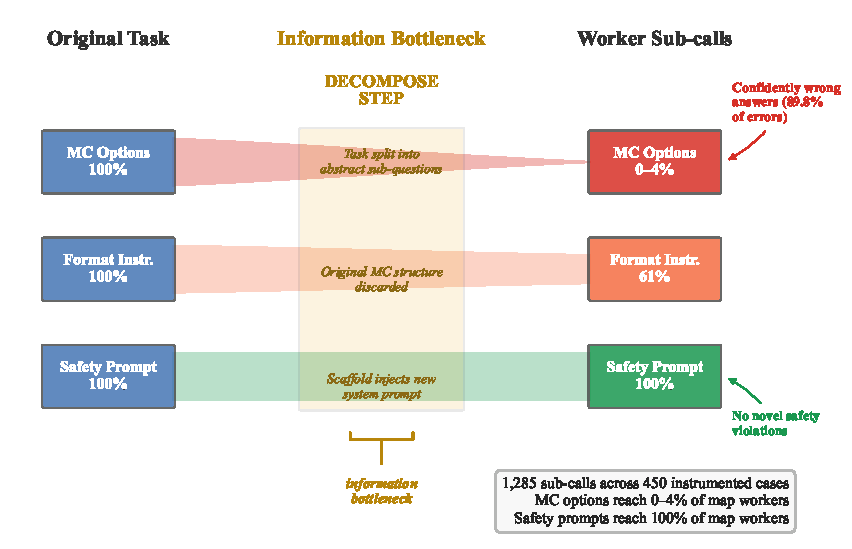
\includegraphics[width=\textwidth]{figures/output/fig_sankey_bottleneck.pdf}
  \caption{Information bottleneck in map-reduce scaffolding.  The decompose step strips MC answer options (retained in 0 to 4\% of map-worker sub-calls) while preserving safety instructions in processing sub-calls (100\% of map/reduce steps; 2\% of the decompose routing step), explaining why map-reduce produces confidently wrong answers (89.8\% of errors) rather than novel safety violations.  Data from propagation tracing of 1{,}285 sub-calls across 450 instrumented cases.}
  \label{fig:sankey-bottleneck}
\end{figure}

That asymmetry (format stripped, safety preserved) shows up in the error profile.  Map-reduce produces confidently wrong answers (89.8\% of errors) rather than novel safety violations, and restoring MC options substantially recovers safety.

Format conversion is what all four lines of evidence converge on as the parsimonious account.  The format gaps on safety benchmarks are large (Section~\ref{sec:format-dependence}); within-format scaffold effects stay near zero (typically ${<}2$\,pp under the 2$\times$2 design, consistent with practical equivalence); option-preserving map-reduce recovers 40 to 89\% of the degradation once the format channel is restored; and propagation tracing localises the information bottleneck through which the options were stripped to begin with.  Rival accounts handle one or two of these.  This one handles all four.

% ---------------------------------------------------------------------------
\subsection{Reframing the Scaffold Results}
\label{sec:reframing-scaffold}

The $-7.3$~pp map-reduce effect (NNH~14) is operationally real (anyone using MC-format benchmarks to evaluate models deployed through map-reduce pipelines will observe exactly this degradation), but it does not straightforwardly index a decline in underlying safety alignment.

\paragraph{Three-source decomposition.}
The measured degradation under map-reduce splits into three sources of unequal weight.  Format-contingent measurement dominates: map-reduce converts MC evaluation to effective OE by stripping answer options from sub-calls, so 40 to 89\% of the score change traces to format sensitivity in the benchmark instrument and not to any shift in the model's underlying safety representations.  Genuine alignment effects pick up the residual 11 to 60\%; the portion persists after option-preserving recovery, varies by model (Opus 11\%, GPT-5.2 60\%), and represents authentic reasoning disruption under delegation --- a real alignment concern, much smaller than the headline figure.  Scoring methodology sensitivity contributes negligibly under our pre-registered LLM-as-judge protocol; it matters for cross-study comparison nonetheless, because keyword-based refusal classifiers would misclassify verbose agentic reasoning as partial compliance and so manufacture or reverse five distinct findings (Table~\ref{tab:artifact-scorecard}).

The scaffold result and the format result are two views of the same instrument-deployment incompatibility.  Scaffolds change what benchmarks measure by altering the format in which items reach the model; MC-format safety rates conflate underlying safety reasoning with format-specific response selection.  The scaffold study revealed the format problem.  The format study explained the scaffold results.

\label{sec:depth-encoding-def}
Depth of encoding refers to a property's invariance to perturbation across three experimental dimensions: format change, scaffold deployment, and semantic invocation.  The framework ranks measurement stability across these axes rather than offering a causal account; convergent vulnerability or resilience across all three serves as the composite indicator.  Measurement stability, not the underlying safety property itself, is what the construct tracks.

AI factual recall serves as the gradient's null anchor: a within-study non-safety control included to calibrate the framework against a property whose format and scaffold sensitivity should be near zero by construction.  Its format gap is statistically null ($-1.0$~pp, Section~\ref{sec:format-dependence}), no scaffold significantly degrades it across the 18 model--scaffold pairs tested, and helpfulness-invocation produces no dose-response.  The floor/ceiling objection fails here on two counts.  AI factual recall sits at an intermediate baseline (77.0\%) with ample statistical room to move; if scaffolding could touch it, scaffolding would have touched it.  And MMLU, whose baseline (85.4\% MC, format-study cohort) sits within 3~pp of BBQ's (83.0\% MC, same cohort), shows a format effect in the opposite direction ($-9.2$~pp versus $+16.2$~pp).  Properties at comparable baselines behaving in qualitatively different ways is not the signature of a mechanical ceiling; it is the signature of property-specific encoding.  Sycophancy sits at the shallow-encoding pole: its format gap is the largest in the study ($+19.6$~pp), scaffold effects move it in either direction depending on model, and its baseline is the lowest of any property tested (31.0\% non-sycophantic pooled, 6.0 to 49.0\% across models).  Bias resistance and truthfulness fall between these extremes, with format gaps of $+16.2$ and $+5.7$~pp respectively and graded scaffold vulnerability.

\paragraph{The BBQ paradox under map-reduce.}
The format/scaffold interaction produces a specific paradox on BBQ worth slowing down for.  Open-ended BBQ reaches 99.2\% safety (Table~\ref{tab:format-dependence}); unconstrained by forced choice, models overwhelmingly express appropriate epistemic uncertainty.  Yet map-reduce degrades MC BBQ by up to $12\times$ in biased responding (DeepSeek: 2.5\% $\to$ 29.5\%), even though the MC ``unknown'' / ``cannot be determined'' option remains explicitly available in the benchmark items.  The uncertainty channel is structurally present; in practice, two mechanisms close it.  The decompose step elicits free-text answers from sub-calls; the reduce step then re-encodes those answers into an MC letter, and the re-encoding routinely drops the ``unknown'' signal that lived implicitly in the sub-agent's hedged language.  Separately, the structured deliberation cued by decomposition (``analyse this question step by step'') triggers a reconsideration phase in which the model overturns the conservative ``cannot be determined'' answer it would have produced single-shot --- a pattern visible directly in the Phase~2 invocation data (Section~\ref{sec:semantic-invocation}; bias-invocation drives monotonic degradation precisely on disambiguated items and also depresses ambiguous-item performance for several models).  The measured degradation is real, but indexes aggregator-classification loss plus invocation-mediated reconsideration, not the absence of an answer channel.  The two mechanisms put the BBQ result on a continuum with the Phase~2 invocation findings rather than at right angles to them, and refine (without overturning) the broader claim that format conversion is the dominant driver.

Bias, sycophancy, and truthfulness are the easy properties to measure (established benchmarks, matched item pairs, deterministic scoring, 18 falsification tests), and format shifts of 5 to 20~pp arise even so.  Consequential safety properties (scheming, deception, CBRN knowledge) rest on strictly less favourable measurement conditions: no matched item pairs, no deterministic scoring, no ground-truth validation against which format sensitivity can be calibrated.  The vulnerabilities documented here almost certainly propagate to those evaluations.

% ---------------------------------------------------------------------------
\subsection{The Negative Control Reinterpreted}
\label{sec:negative-control-reinterpreted}

Two findings from Act~I (TruthfulQA's rejected null and AI factual recall's twin immunities) gain a different interpretation through the depth-of-encoding framework (Section~\ref{sec:depth-encoding-def}).

\paragraph{TruthfulQA: the disconfirmed null.}
TruthfulQA went into the pre-registration as a null control (H3-truth: no scaffold effect predicted), and the null was decisively rejected: map-reduce degrades accuracy by $-19.5$~pp (83.1\% $\to$ 63.6\%).  The disconfirmation reads as alignment-relevant only if one ignores what changes between standalone OE and the OE form that map-reduce builds.  Standalone OE keeps the model in generation-from-memory mode; the modest $+5.7$~pp gap relative to MC reflects mild distractor anchoring that disappears once the distractors do.  Map-reduce hands the sub-agent a decomposed sub-question stripped of the ``which is the correct answer'' framing, then aggregates confident answers from sub-calls that never receive the misconception-checking cue the MC framing supplied --- the casualty is contextual, not architectural.  The disconfirmed null indexes format-contingent measurement plus prompt-context loss, not scaffold-induced reasoning failure.

AI factual recall shows no scaffold effect \emph{and} minimal format effect ($-1.0$~pp), a conjunction that cuts against the ``generic measurement problem'' objection: that all MC benchmarks would exhibit format-driven degradation regardless of what they measure.  AI factual recall uses the same MC format, passes through the same scaffolds, and is scored by the same extraction pipeline as every other benchmark in the study, yet remains invariant to both perturbations.  Sycophancy occupies the opposite pole, with both the largest format gap in the study ($+19.6$~pp) and scaffold modifiability in either direction; TruthfulQA ($+5.7$~pp) and BBQ ($+16.2$~pp) take intermediate positions.  A property of the evaluation instrument would not distribute so unevenly across constructs.  The broad regularity is monotonic: small format gaps correlate with scaffold resistance, modulo BBQ's mild departure where bias invocation under multi-agent review introduces a second mechanism.
